\begin{frame}{Visualization of fANOVA components under Dependence} % How does it look?
  \begin{align*}
    y(x_1, x_2) = 2x_1 + x_2^{2} + x_1 x_2, \qquad \rho = 0.8
  \end{align*}
  \begin{columns}
    \column{0.5\textwidth}
      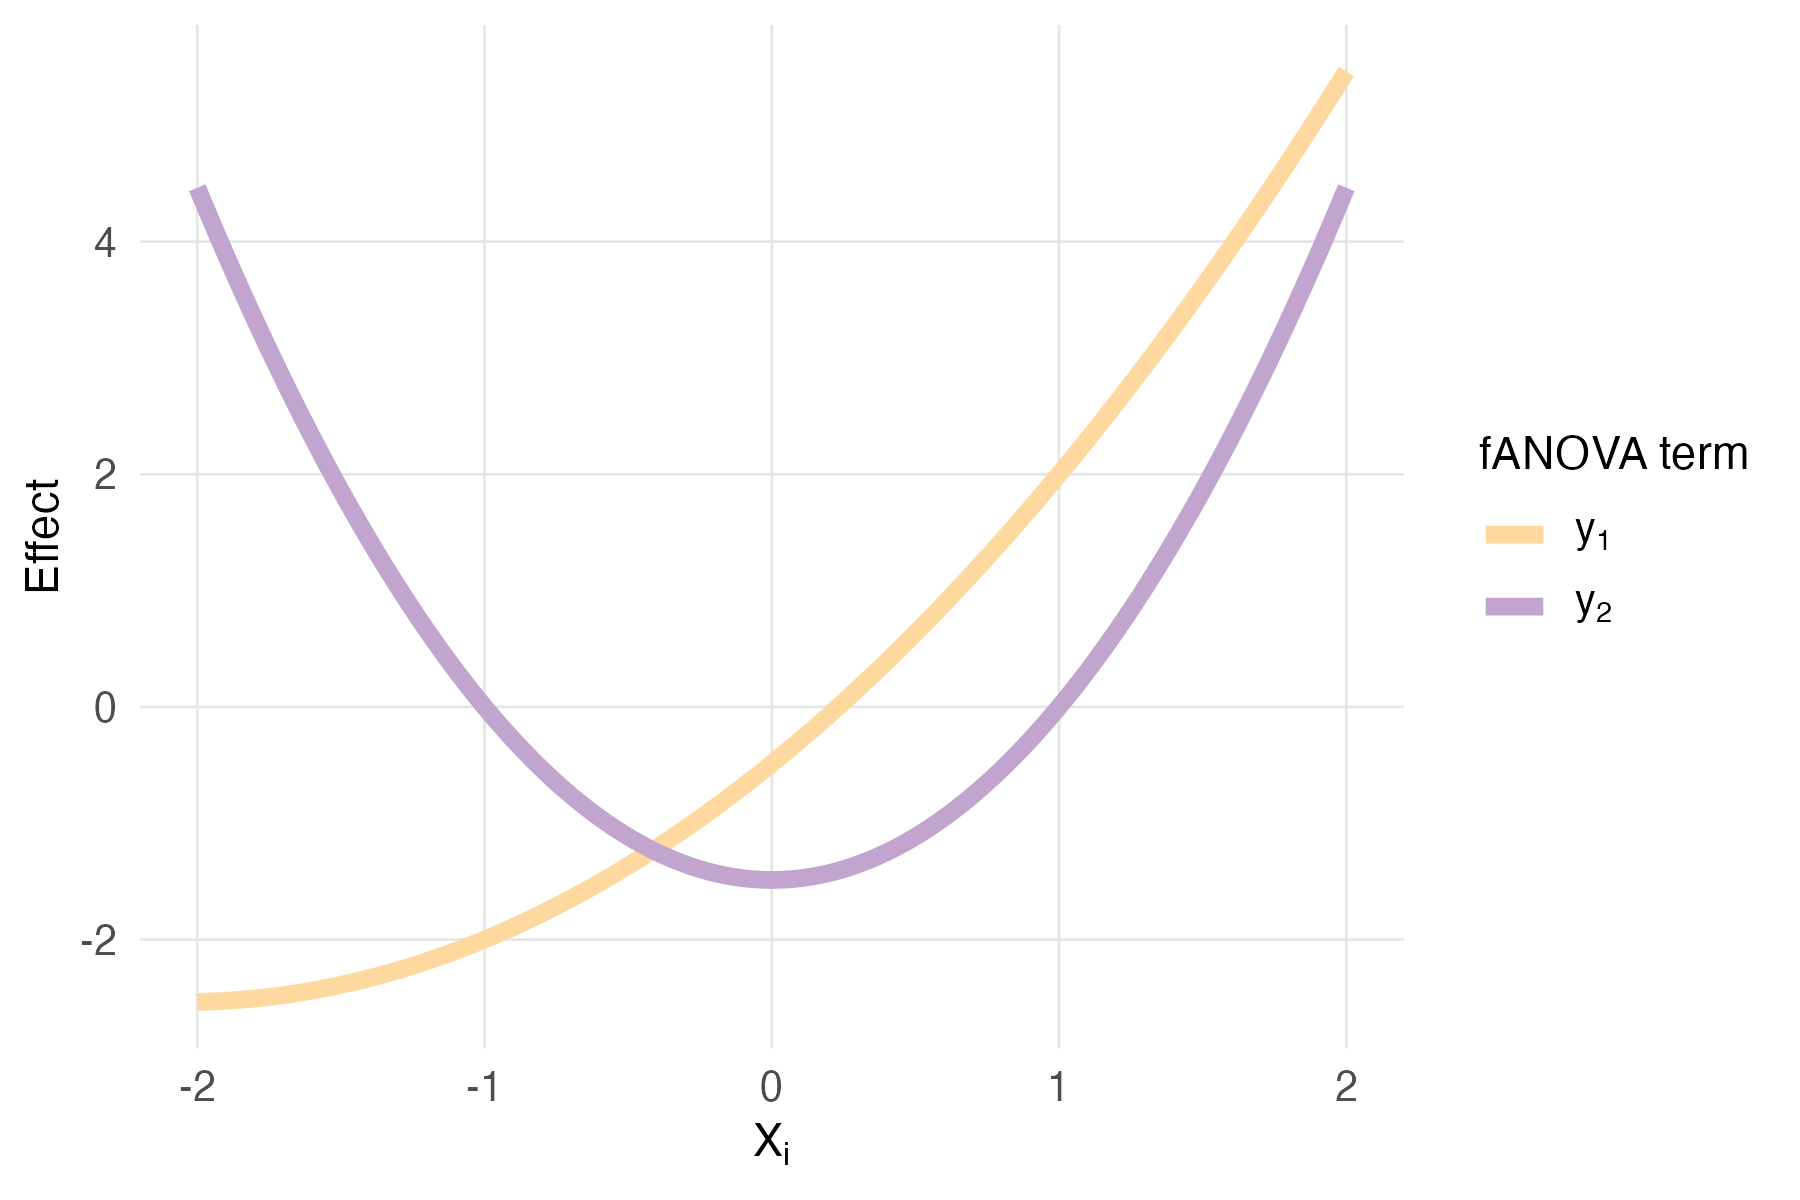
\includegraphics[width=\linewidth]{../images/experiment_section/gen_ex_1_a1p20_a2p00_a11p00_a22p10_a12p10_rhop08_main.png}
    \column{0.5\textwidth}
      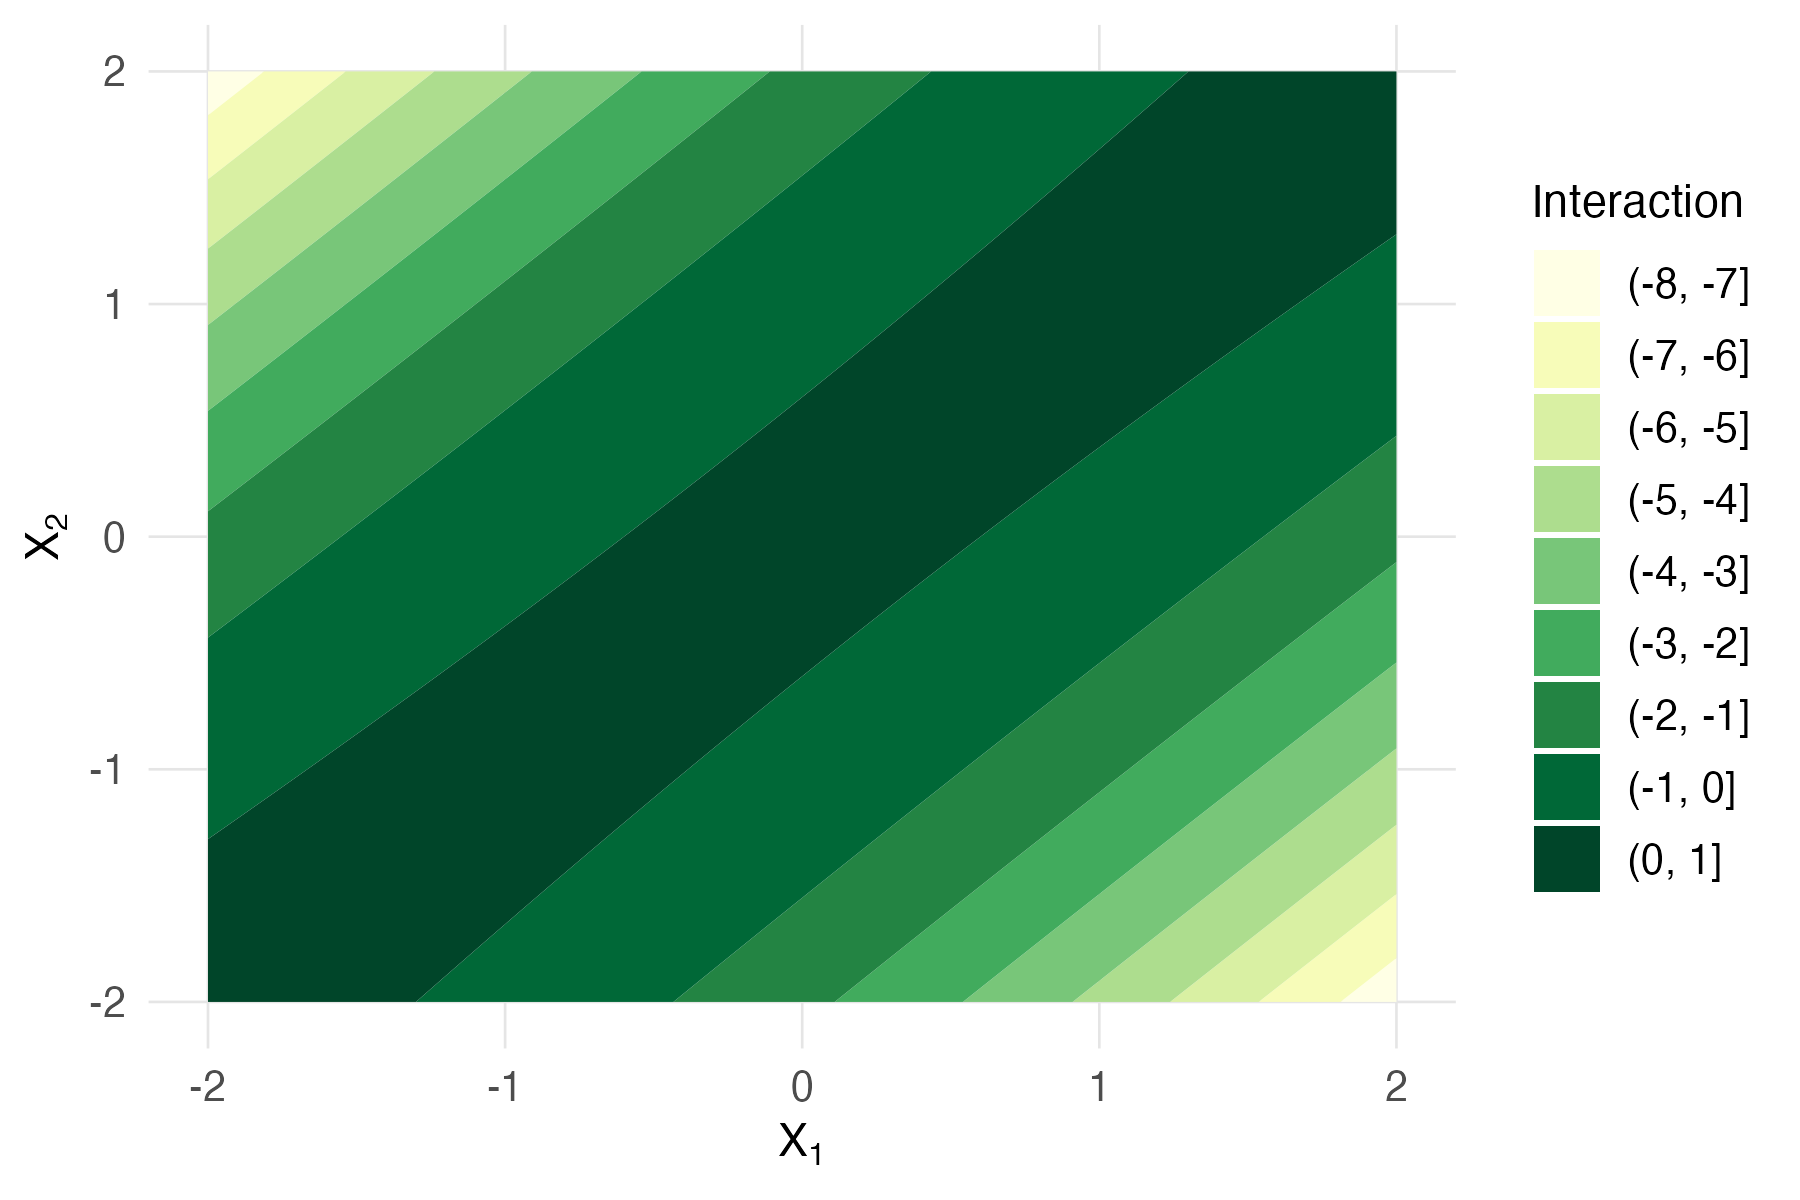
\includegraphics[width=\linewidth]{../images/experiment_section/gen_ex_1_a1p20_a2p00_a11p00_a22p10_a12p10_rhop08_interaction.png}
  \end{columns}
\end{frame}

%==================================================
% Slide 2 – Conditions (Weaker Annihilating Conditions)
%==================================================
\begin{frame}{Conditions for Interpretability under Dependent Inputs}
  \begin{block}{Weak Annihilating Conditions}
    \uncover<1->{
\begin{equation*}
    \int_{\mathbb{R}} y_{u, G}(\boldsymbol{x}_u) f_{\boldsymbol{u}}(\boldsymbol{x}_u) d\nu (x_i) = 0 \quad \text{for} \quad i \in u \neq \emptyset
\end{equation*}
    }
  \end{block}

    \begin{itemize}
    \item<2-> $f_{\{i\}}$ : marginal density of variable $X_u$ (possibly multivariate)
  \end{itemize}

  \uncover<2->{It follows:}

  \uncover<3->{
    \[
      \mathbb{E}[y_{u, G}(\boldsymbol{X}_u)] 
      := \int_{\mathbb{R}^N} 
          y_{u, G}(\boldsymbol{x}_u) 
          f_{\boldsymbol{X}}(\boldsymbol{x}) 
          \, d\nu (\boldsymbol{x}) 
        = 0
    \]
  }

  \uncover<4->{
    \[
      \mathbb{E}[y_{u, G}(\boldsymbol{X}_u) 
                 y_{v, G}(\boldsymbol{X}_v)] 
      := \int_{\mathbb{R}^N} 
          y_{u, G}(\boldsymbol{x}_u) 
          y_{v, G}(\boldsymbol{x}_v) 
          f_{\boldsymbol{X}}(\boldsymbol{x}) 
          \, d\nu (\boldsymbol{x}) 
        = 0 
        \quad (v \subsetneq u)
    \]
  }
\end{frame}




\begin{frame}{Generalized Components Mirror the Classical Form}
\begin{align*}
    % --- constant term (always visible)
    y_{\emptyset,G} 
      &= \int_{\mathbb{R}^N} y(\boldsymbol{x}) 
         f_{\boldsymbol{X}}(\boldsymbol{x}) \, d \nu(\boldsymbol{x}) \\[3ex]
    % --- nonconstant formula (appears from slide 2 onward)
    \onslide<2->{%
    y_{u,G}(\boldsymbol{X}_u) 
      &= \int_{\mathbb{R}^{N - |u|}} 
         y(\boldsymbol{X}_u, \boldsymbol{x}_{-u})
         f_{-u}(\boldsymbol{x}_{-u})\, d \nu(\boldsymbol{x}_{-u}) 
         \textcolor<3->{pastelRedDark}{-\sum_{v \subsetneq u} y_{v,G}(\boldsymbol{X}_v)} \\ 
      &\quad 
        \textcolor<4->{pastelBlueDark}{
        -\!\!\!\!\!\!\sum_{\substack{\emptyset \ne v \subseteq \{1,\dots,N\} \\ 
        v \cap u \ne \emptyset,\ v \not\subset u}} 
        \int_{\mathbb{R}^{|v \cap -u|}} 
        y_{v,G}(\boldsymbol{X}_{v \cap u}, \boldsymbol{x}_{v \cap -u}) 
        f_{v \cap -u}(\boldsymbol{x}_{v \cap -u}) 
        \, d \nu(\boldsymbol{x}_{v \cap -u})}
    }
  \end{align*}
\begin{itemize}
  \item<3-> \textcolor{pastelRedDark}{$u = \{1\}$ $\rightarrow$ $v \subsetneq u \in \{\emptyset\}$}
  \item<4-> \textcolor{pastelBlueDark}{$(\emptyset \ne v \subseteq \{1,\dots,N\},\ v \cap u \ne \emptyset,\ v \not\subset u) \in \{\{1,2\}, \{1,3\}, \{1,2,3\}\}$}
\end{itemize}

\end{frame}


\begin{frame}{Coupled System of Generalized Components}
    \begin{itemize}
    \item $N = 3$, $u = \emptyset$
  \end{itemize}
    \begin{equation*}
    y_{\emptyset,G} = \mathbb{E}[y(\boldsymbol{X})]
    \end{equation*}
    \begin{itemize}
      \item \textcolor{pastelRedDark}{$u = \{1\}$ $\rightarrow$ $v \subsetneq u \in \{\emptyset\}$} and \textcolor{pastelBlueDark}{$(\emptyset \ne v \subseteq \{1,\dots,N\},\ v \cap u \ne \emptyset,\ v \not\subset u) \in \{\{1,2\}, \{1,3\}, \{1,2,3\}\}$}
    \end{itemize}
    \begin{align*}
       y_{{\{1\}},G}(\boldsymbol{X}_u) &= \int_{\mathbb{R}^{2}} y(x_1, x_2, x_3) f_{{\{2, 3\}}}(x_2, x_3) \, d \nu(x_2, x_3) - y_{\emptyset,G} \\[1em]
    &\quad - \int_{\mathbb{R}}y_{{\{1, 2\}}, G}(x_1, x_2)f_{{\{2\}}}(x_2) \, d \nu(x_2) - \int_{\mathbb{R}}y_{{\{1, 3\}}, G}(x_1, x_3)f_{{\{3\}}}(x_3) \, d \nu(x_3) \\[1em]
    &\quad - \int_{\mathbb{R}^2}y_{{\{1, 2, 3\}}, G}(x_1, x_2, x_3)f_{{\{2, 3\}}}(x_2, x_3) \, d \nu(x_2, x_3)
    \end{align*}
\end{frame}


\begin{frame}{Coupled System of Generalized Components}
      \begin{itemize}
      \item \textcolor{pastelRedDark}{$u = \{1, 2\}$ $\rightarrow$ $v \subsetneq u \in \{\emptyset\,, \{1\}, \{2\}\}$} and \textcolor{pastelBlueDark}{$(\emptyset \ne v \subseteq \{1,\dots,N\},\ v \cap u \ne \emptyset,\ v \not\subset u) \in \{\{1,2,3\}\}$}
    \end{itemize}
    \begin{align*}
       y_{{\{1, 2\}},G}(\boldsymbol{X}_u) &= \int_{\mathbb{R}} y(x_1, x_2, x_3) f_{{\{3\}}}(x_3) \, d \nu(x_3) - y_{\emptyset,G} - y_{{\{1\}},G} - y_{{\{2\}},G}\\[1em]
    &\quad - \int_{\mathbb{R}}y_{{\{1, 2, 3\}}, G}(x_1, x_2, x_3)f_{{\{3\}}}(x_3) \, d \nu(x_3)
    \end{align*}
\end{frame}


\begin{frame}{Coupled System of Generalized Components}
      \begin{itemize}
      \item \textcolor{pastelRedDark}{$u = \{1, 2, 3\}$ $\rightarrow$ $v \subsetneq u \in \{\emptyset\,, \{1\}, \{2\}, \{3\}, \{1, 2\}, \{1, 3\}, \{2, 3\}\}$} and \textcolor{pastelBlueDark}{\(\nexists v \subseteq \{1,\dots,N\} \ \text{s.t.} \ v \neq \emptyset, \ v \cap u \neq \emptyset, \ v \nsubseteq u\)
}
    \end{itemize}
    \begin{align*}
       y_{{\{1, 2, 3\}},G}(\boldsymbol{X}_u) &= y(x_1, x_2, x_3) - y_{\emptyset,G}\\[1em]
    &\quad - y_{{\{1\}},G} - y_{{\{2\}},G} - y_{{\{3\}},G} \\[1em]
    &\quad - y_{{\{1, 2\}},G} - y_{{\{1, 3\}},G} - y_{{\{2, 3\}},G}
    \end{align*}
\end{frame}

\begin{frame}{Construction of Components via Fourier-polynomial Expansion}
\begin{align*}
    \onslide<1->{%
    y(x_1,x_2) 
    &= a_0 + a_1 x_1 + a_2 x_2 
       + a_{11} x_1^2 + a_{22} x_2^2 + a_{12} x_1 x_2 
    } \\[0.5em]
    \onslide<2->{%
    &= c_0 
       + c_{1,1}\,\psi_{1,1}(x_1) 
       + c_{2,1}\,\psi_{2,1}(x_2) 
    } \\[0.5em]
    \onslide<3->{%
    &\quad
       + c_{1,2}\,\psi_{1,2}(x_1)
       + c_{2,2}\,\psi_{2,2}(x_2)
       + c_{12,11}\,\psi_{12,11}(x_1,x_2) 
    } \\[0.5em]
    \onslide<4->{%
    &= 
       \underbrace{c_0}_{y_0}
       + \underbrace{\big(c_{1,1}\,\psi_{1,1}(x_1) 
                         + c_{1,2}\,\psi_{1,2}(x_1)\big)}_{y_1(x_1)} 
    } \\[0.5em]
    \onslide<5->{%
    &\quad
       + \underbrace{\big(c_{2,1}\,\psi_{2,1}(x_2) 
                         + c_{2,2}\,\psi_{2,2}(x_2)\big)}_{y_2(x_2)} 
    } \\[0.5em]
    \onslide<6->{%
    &\quad
       + \underbrace{c_{12,11}\,\psi_{12,11}(x_1,x_2)}_{y_{12}(x_1,x_2)}
    }
\end{align*}

\end{frame}

\begin{frame}{Choosing Orthogonal Basis Functions}
  For Gaussian input variables Hermite polynomial basis functions are proposed:
  \begin{align*}
    \psi_{\emptyset}(x_1,x_2) &= 1, \\[0.5em]
\psi_{1,1}(x_1) &= x_1, \\[0.5em]
\psi_{2,1}(x_2) &= x_2, \\[0.5em]
\psi_{1,2}(x_1) &= x_1^2 - 1, \\[0.5em]
\psi_{2,2}(x_2) &= x_2^2 - 1, \\[0.5em]
\psi_{12,11}(x_1,x_2) &= \frac{\rho (x_1^2 + x_2^2)}{1 + \rho^2} 
                         - x_1 x_2 
                         + \frac{\rho(\rho^2 - 1)}{1 + \rho^2}
\end{align*}
\end{frame}


\begin{frame}{fANOVA Components of a two-degree Polynomial}
  \begin{itemize}
    \item Yields fANOVA components for Gaussian Inputs
    \item Works for polynomials of degree up to $d = 2$
  \end{itemize}
  \begin{align*}
\begin{split}
y_{\emptyset, G} &= a_0 + a_{11} + a_{22} + \rho\,a_{12}, \\[0.5em]
y_{\{1\}, G}(x_1) &= a_1\,x_1 
  + \left(a_{11} + \frac{\rho}{1+\rho^2}a_{12}\right)\bigl(x_1^2 - 1\bigr), \\[0.5em]
y_{\{2\}, G}(x_2) &= a_2\,x_2 
  + \left(a_{22} + \frac{\rho}{1+\rho^2}a_{12}\right)\bigl(x_2^2 - 1\bigr), \\[0.5em]
y_{\{1,2\}, G}(x_1,x_2) 
&= -a_{12}\!\left(
    \frac{\rho(x_1^2+x_2^2)}{1+\rho^2} 
    - x_1 x_2 
    + \frac{\rho(\rho^2-1)}{1+\rho^2}
   \right)
\end{split}
\end{align*}
\end{frame}
  

\begin{frame}{Decomposition under Weak Correlation}
    \[
    z(x_1, x_2) = 2x_1 + x_1^2 + 0.5 x_1 x_2
    \]
  \begin{columns}
    \column{0.5\textwidth}
      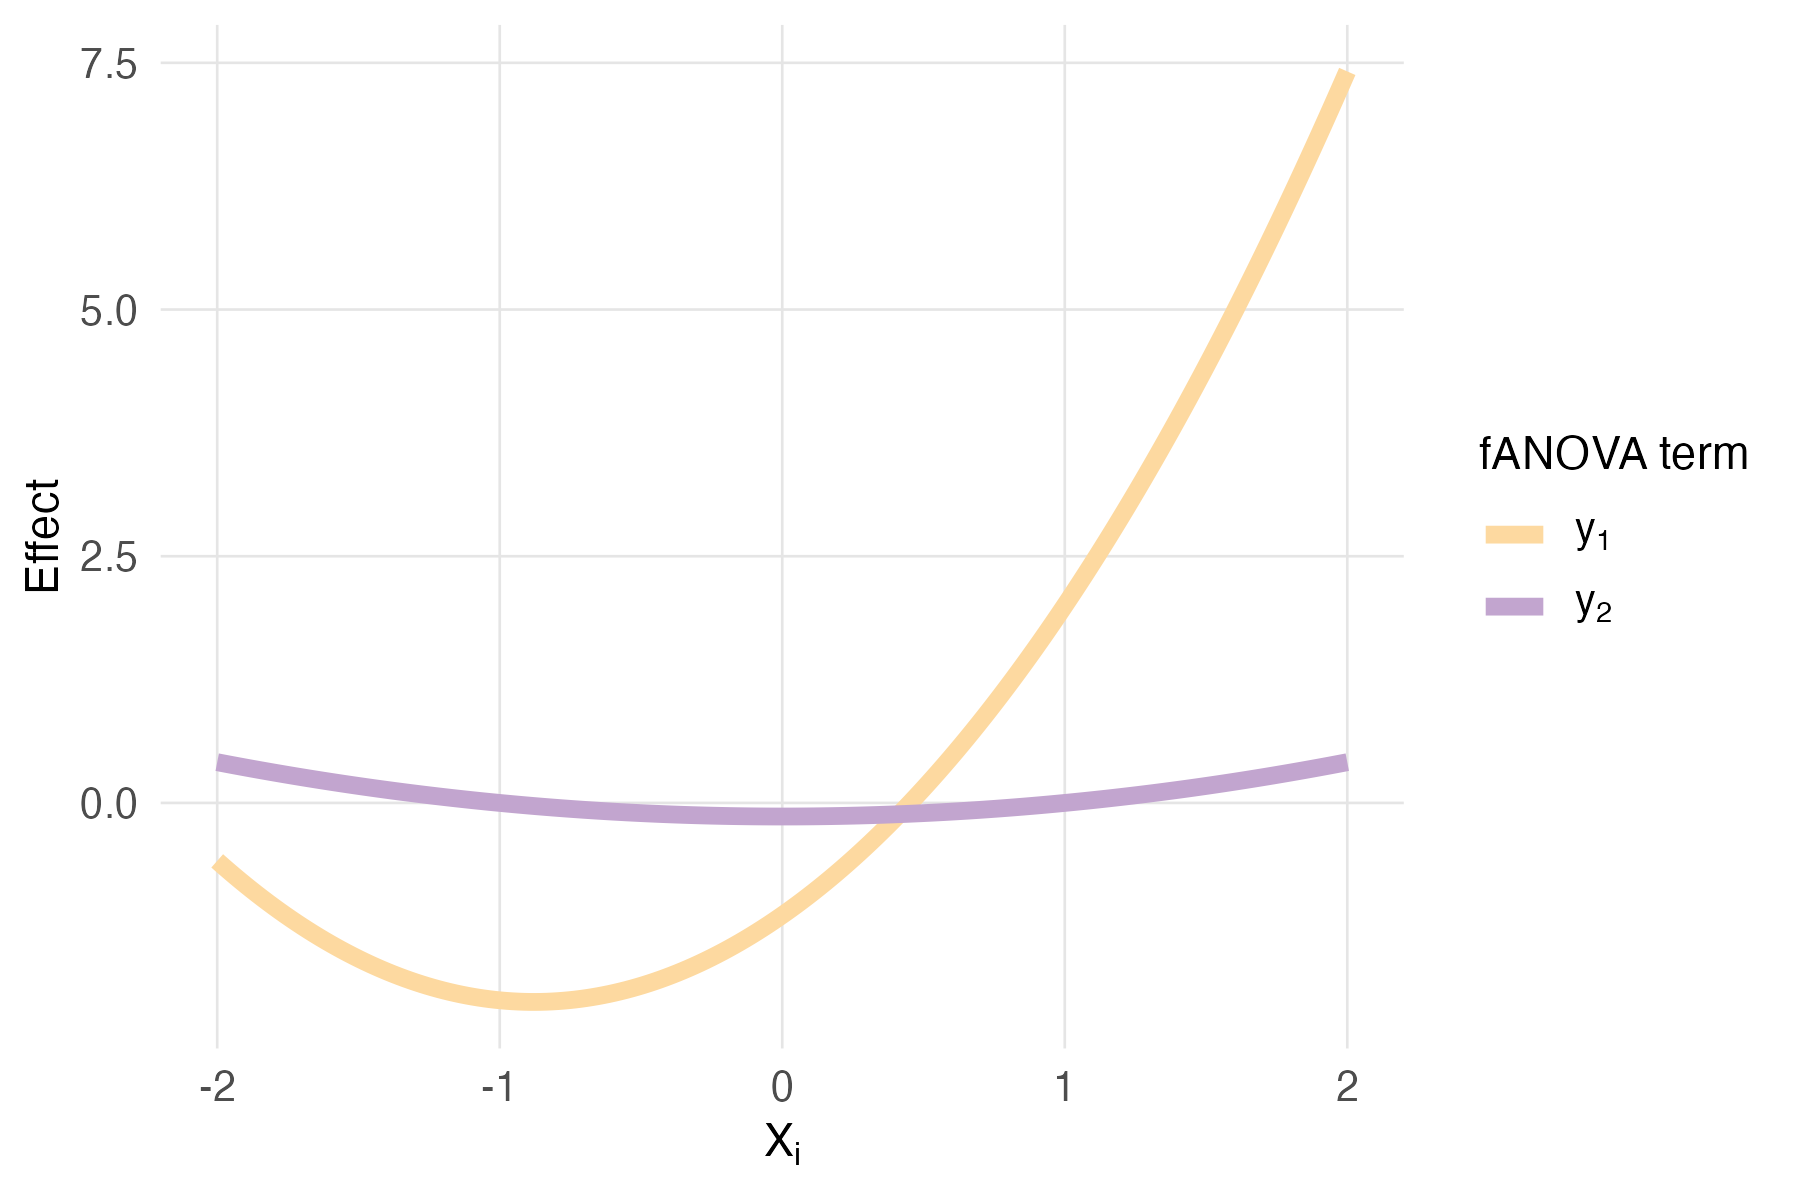
\includegraphics[width=\linewidth]{../images/experiment_section/full_a1p20_a2p00_a11p10_a22p00_a12p05_rhop03_main.png}
      \captionof{figure}{Main effect for $\rho = 0.3$.}
    \column{0.5\textwidth}
      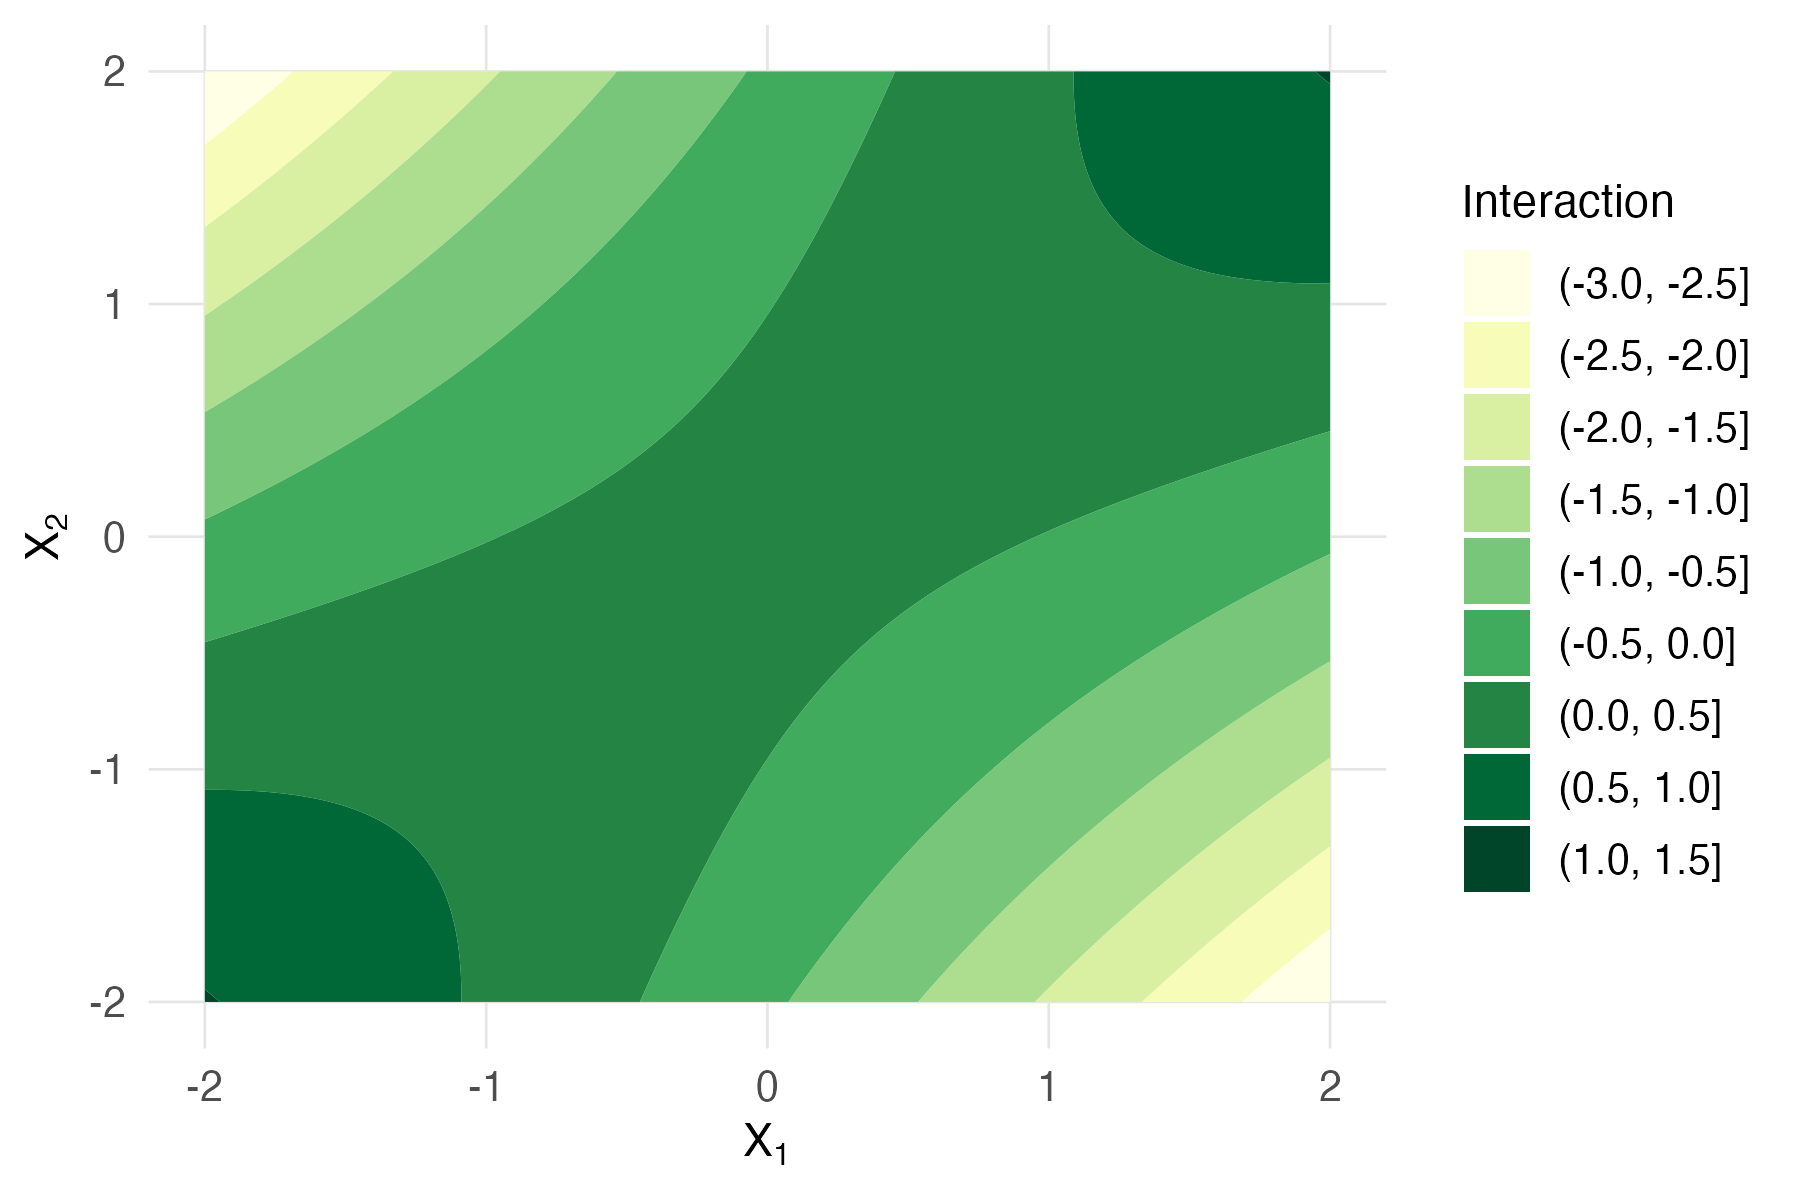
\includegraphics[width=\linewidth]{../images/experiment_section/full_a1p20_a2p00_a11p10_a22p00_a12p05_rhop03_interaction.png}
      \captionof{figure}{Interaction effect for $\rho = 0.3$.}
  \end{columns}
  
\end{frame}

\begin{frame}{Decomposition under Independence}
    \[
    z(x_1, x_2) = 2x_1 + x_1^2 + 0.5 x_1 x_2
    \]
  \begin{columns}
    \column{0.5\textwidth}
      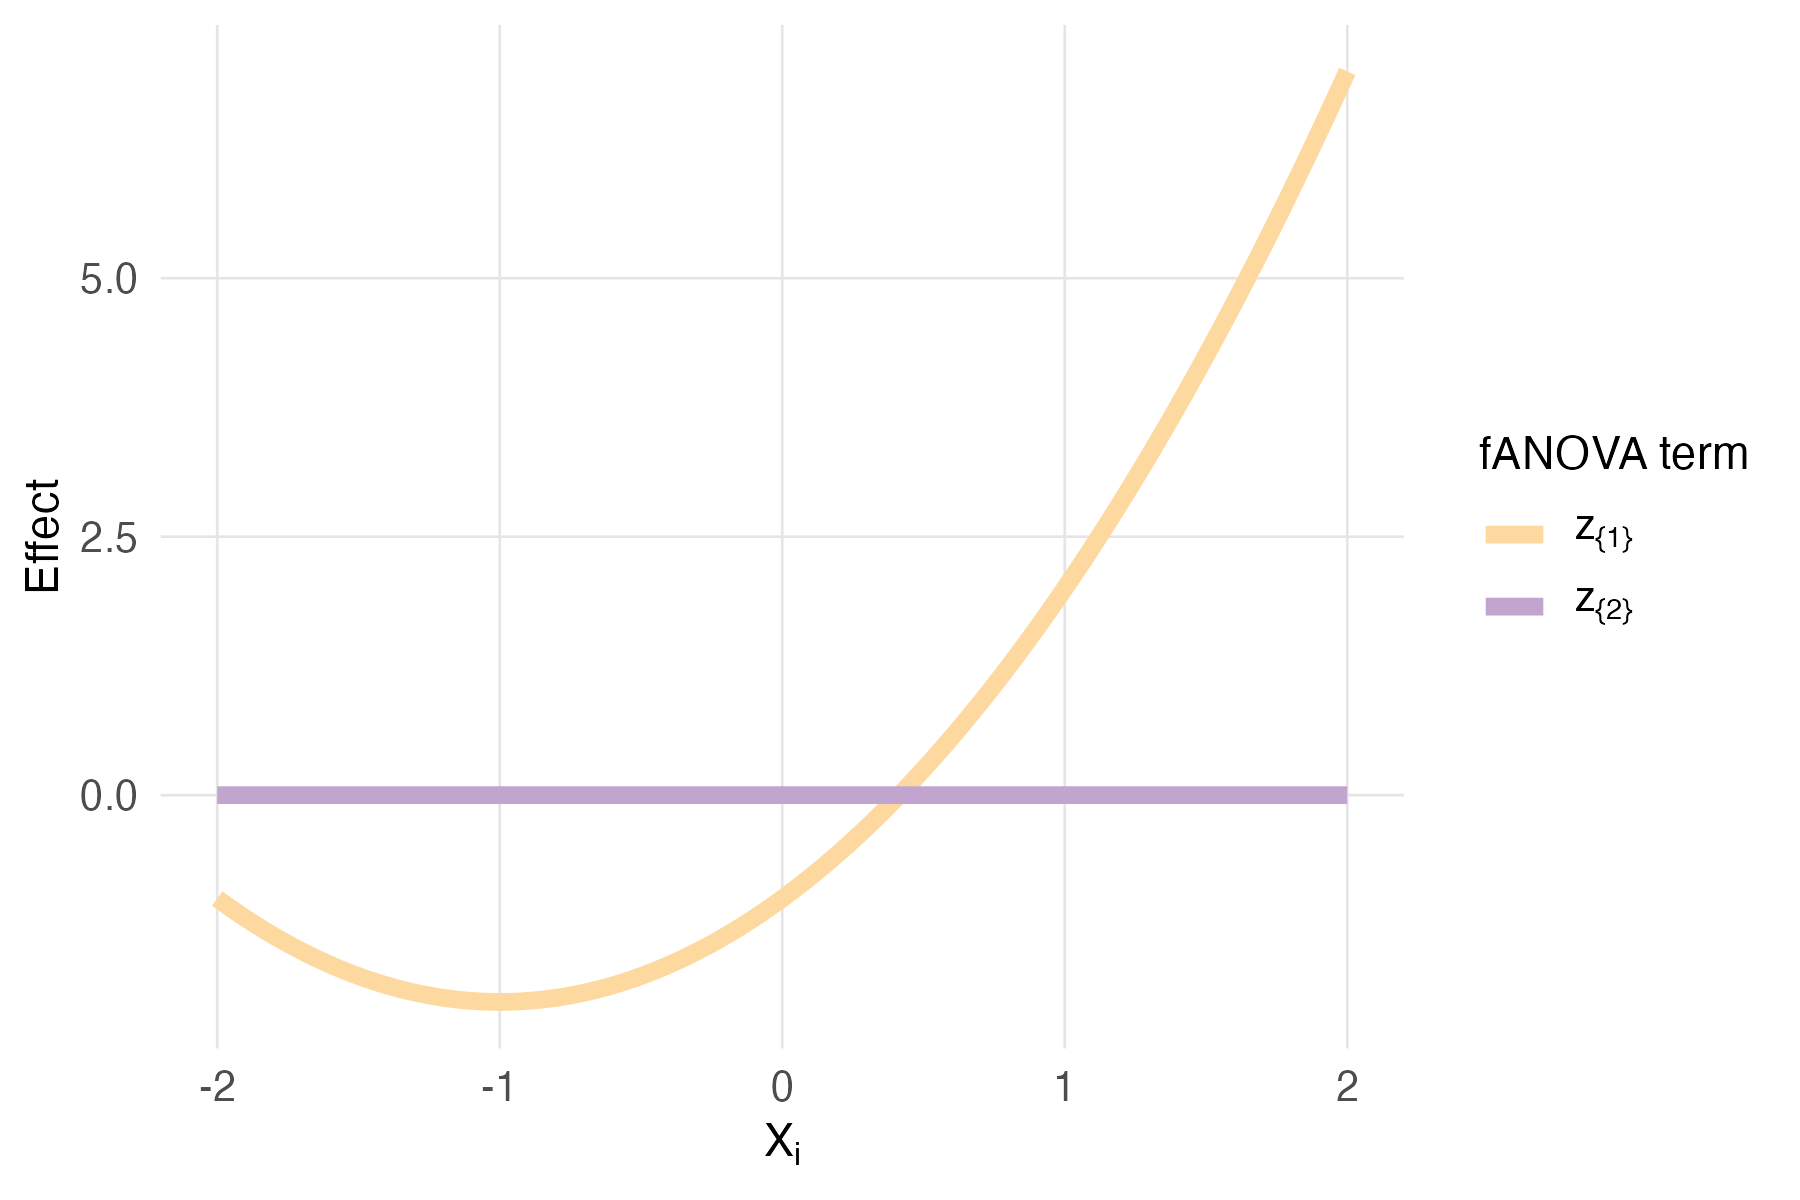
\includegraphics[width=\linewidth]{../images/experiment_section/full_a1p20_a2p00_a11p10_a22p00_a12p05_rhop00_main.png}
      \captionof{figure}{Main effect for $\rho = 0$.}
    \column{0.5\textwidth}
      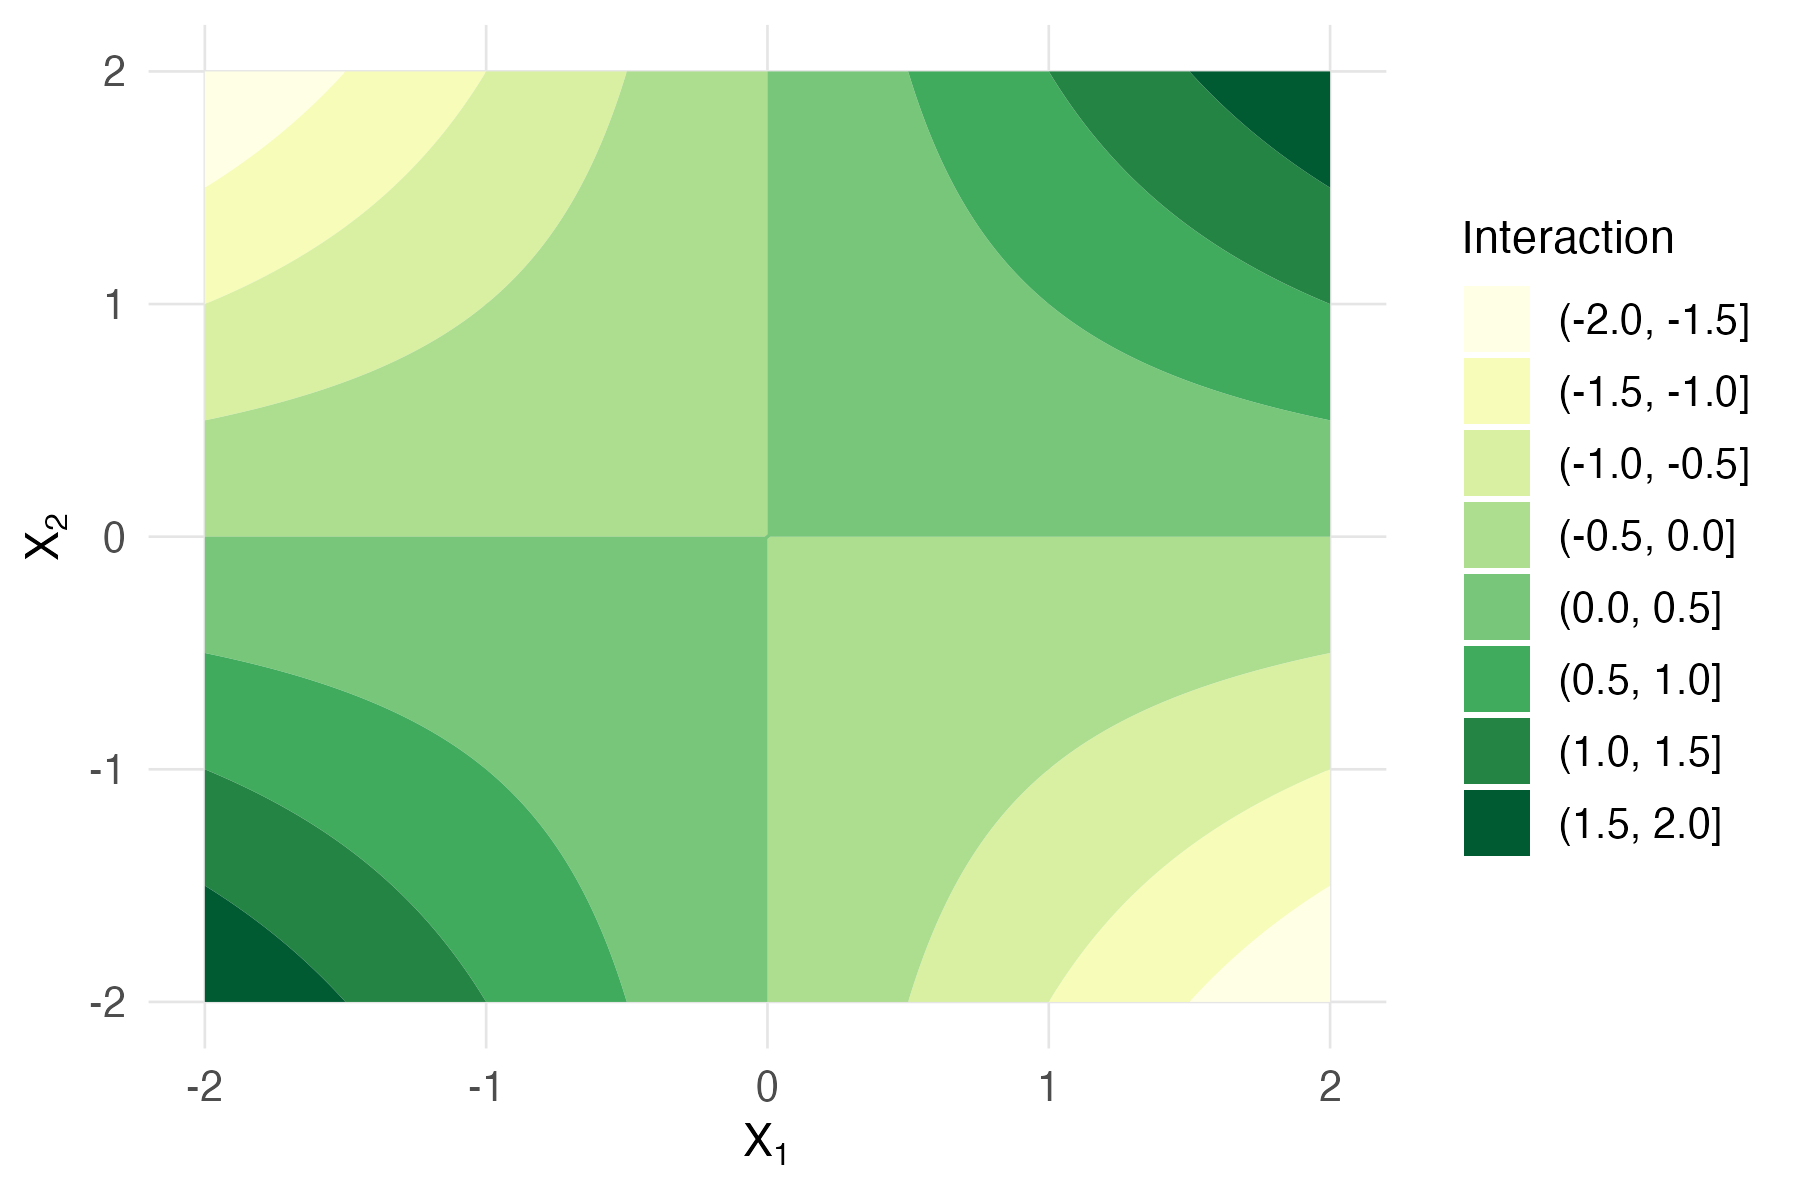
\includegraphics[width=\linewidth]{../images/experiment_section/full_a1p20_a2p00_a11p10_a22p00_a12p05_rhop00_interaction.png}
      \captionof{figure}{Interaction effect for $\rho = 0$.}
  \end{columns}
  \[
  \Rightarrow \text{nonzero main effect of } X_2 \text{ only present under correlation.}
  \]
\end{frame}




\begin{frame}{Variance Decomposition via fANOVA}
  Not only $y$, but also its variance can be decomposed:
\begin{align*}
    \onslide<1->{\mu &:= \mathbb{E}[y(\boldsymbol{X})] = y_{\emptyset,G}} \\[1em]
    \onslide<2->{\sigma^2 
    &:= \mathbb{E}\left[ \left( y(\boldsymbol{X}) - \mu \right)^2 \right]} \\[0.5em]
    \onslide<3->{&= \mathbb{E} \left[ \left( y_{\emptyset,G} + \sum_{u} y_{u,G}(\boldsymbol{X}_u) - y_{\emptyset,G} \right)^2 \right]} \\[0.5em]
    \onslide<4->{&= \mathbb{E} \left[ \left( \sum_{u} y_{u,G}(\boldsymbol{X}_u) \right)^2 \right]} \\[0.5em]
    \onslide<5->{&= \sum_{u} \mathbb{E} \left[ y_{u,G}^2(\boldsymbol{X}_u) \right]
    + \sum_{\substack{u \not\subseteq v,\, v \not\subseteq u}} 
    \mathbb{E} \left[ y_{u,G}(\boldsymbol{X}_u) y_{v,G}(\boldsymbol{X}_v) \right]}
\end{align*}

\end{frame}


\begin{frame}{Alternative Generalization of fANOVA}
  Different formulations of generalized fANOVA components exists, e.g.:
    \begin{align*}
\left\{ y_{u, G}(\boldsymbol{x}_u) \,\middle|\, u \subseteq d \right\}
= \arg\min_{\{g_u \in \mathcal{L}^2(\mathbb{R}^{|u|})\}} 
\int_{\mathbb{R}^N} \left( \sum_{u \subseteq d} g_u(\boldsymbol{x}_u) - y(\boldsymbol{x}) \right)^2 
f_{\boldsymbol{X}}(\boldsymbol{x}) \, d \nu (\boldsymbol{x}),
\label{eq:generalized_fanova_components_hooker}
\end{align*}
subject to hierarchical orthogonality conditions:
\begin{align*}
    \forall v \subseteq u,\ \forall g_v:\ 
    \int_{\mathbb{R}^N} y_u(\boldsymbol{x}_u) g_v(\boldsymbol{x}_v) 
    f_{\boldsymbol{X}}(\boldsymbol{x}) \, d \nu (\boldsymbol{x}) = 0.
\end{align*}
\end{frame}
